\documentclass[a4j,twocolumn,dvipdfmx,uplatex]{jsarticle}
%\documentclass[a4j,twocolumn]{jarticle} % 'jsarticle' が使えない場合はこちらを利用

% 上記 documentclass のオプションは自由に追加してもよい.

%%%%%%%%%%%%%%%%%%%%%%%%%%%%%%%%%%%%%%%%%%%%%%%%%%%%%%%%%%%%%%%%%%%%%%%%%%%%%%
%%% ページ設定 (この項目は論文著者は編集しないこと.)

% 芸術科学会論文誌用スタイルパッケージ
\usepackage{artsci-jour-j}

% 開始ページ数設定
\setcounter{page}{1234}

% ヘッダスタイル
\markright{\footnotesize{
\textbf{芸術科学会論文誌 Vol. 1, No. 5, pp. 1234 -- 1236 (2015)}
}}
\pagestyle{myheadings}

%%%%%%%%%%%%%%%%%%%%%%%%%%%%%%%%%%%%%%%%%%%%%%%%%%%%%%%%%%%%%%%%%%%%%%%%%%%%%%
%%% パッケージ一覧 (必要なパッケージを任意に追加してよい)

\usepackage{amsmath, amssymb}	% AMS-LaTeX
\usepackage[dvipdfmx]{graphicx}	% 「graphics」パッケージに変更してもよい.
\graphicspath{{./figs/}{./suppl/}}         	% グラフィックを置いたディレクトリを自動で補完する
\usepackage{float}			% 図表が記述位置から飛ばないためのパッケージ
\usepackage{comment} 			% ブロックコメントを作成する
\usepackage[switch,columnwise]{lineno} 	% 行番号表示(主に添削用)


%%%%%%%%%%%%%%%%%%%%%%%%%%%%%%%%%%%%%%%%%%%%%%%%%%%%%%%%%%%%%%%%%%%%%%%%%%%%%%
%%% マクロ一覧 (必要なマクロをこの部分に記述)

\newcommand{\bA}{\mathbf{A}}
\newcommand{\bB}{\mathbf{B}}

%% src path を勝手に include する
\makeatletter
\providecommand*{\input@path}{}
\g@addto@macro\input@path{{./src/}{./suppl/}}% append
\makeatother

%%%%%%%%%%%%%%%%%%%%%%%%%%%%%%%%%%%%%%%%%%%%%%%%%%%%%%%%%%%%%%%%%%%%%%%%%%%%%%
%%% タイトル,著者,所属,概要
%%%%%%%%%%%%%%%%%%%%%%%%%%%%%%%%%%%%%%%%%%%%%%%%%%%%%%%%%%%%%%%%%%%%%%%%%%%%%%
%%% タイトル,著者,所属,概要
% 日本語タイトル
\jtitle{
芸術科学会論文誌サンプル(\LaTeX 版) % タイトル記述.適宜改行を入力.
}

% 英語タイトル
\etitle{
A Sample for the Journal of the Society for Art and Science \\
(\LaTeX Version)
}

% 日本語著者
% 所属参照は好みに応じて \dagger などを用いてもよい.
\jauthor{
芸術科学太郎\(^{1)}\){\small (学生会員)}
~~~ % 氏名の間隔はチルダ記号や hspace 等で適宜調節のこと.
芸術科学次郎\(^{2)}\){\small (正会員)}
}

% 英語著者
\eauthor{
Taro Geijutsu-Kagaku\(^{1)}\)
~~~
Jiro Geijutsu-Kagaku\(^{2)}\)
}

% 日本語所属
\jaffiliation{
1) 芸術科学大学大学院芸術科学研究科
~~~
2) 芸術科学大学芸術科学部
}

% 英語所属
\eaffiliation{
1) Graduate School of Art and Science, The University for Art and Science\\
2) Department of Art and Science, The University for Art and Science
}

% 連絡先電子メールアドレス(省略可)
% (スパム対策は著者自身の判断によって措置すること.
% このサンプルでは「@」を2バイト文字にすることで対応してある.)
\email{
\{taro, jiro\}@art-science.ac.jp
}


% 日本語概要
% 英語概要
% 日本語概要
\jabstract{
本稿は,芸術科学会論文誌の投稿用のLaTeX版サンプルを提供するものである.
}

% 英語概要
\eabstract{
This paper presents the LaTeX version of a sample for the Journal
of the Society for Art and Science.
}



%%%%%%%%%%%%%%%%%%%%%%%%%%%%%%%%%%%%%%%%%%%%%%%%%%%%%%%%%%%%%%%%%%%%%%%%%%%%%%
% ここより論文本体

\begin{document}
\maketitle
\thispagestyle{myheadings}

%% ここで改ページし,以降の本文は2カラムとする
\clearpage % もし2ページ目が空白ページになるなら,ここをコメントアウト

% はじめに
\section{はじめに}

画材としての煤は古代より広く利用されている.煤をそのまま利用する,あるいは
煤をあつめ黒い塗料として利用することで絵画を描画することは広く行われている.

蝋燭の煤を利用し,直接すすを画材に塗布することで描画する方法も広く行われており,
数々の作品が発表されている.

筆者らは
煤の持つ光を反射しない黒色の色
煤の付着する様子
蝋燭の炎の揺らぎ
などに着目し sootoid\cite{sootid}を作成した.
しかしながら,機構の制約として煤を塗布する太さに
自然のゆらぎ以上の変化をもたらせないこと,途中での消火・点火を行わないため
一筆書きとなるような画像しか描画できないことなどの課題が残った.

本研究ではこれらの課題に着目し,新たに煤生成の制御機構を構築することで
より表現力の豊かなさまざまな種類の描画を可能としたものである.



% 途中のファイル名は論文にあわせて考ええよう
% 以下は論文の書き方です.
\section{投稿論文の書式}

\subsection{ページ設定およびページ数}

論文本体のページ設定は,A4とする.このページ設定で不都合なコンテンツがある場合は,
静止画であっても論文本体に含めずに添付ファイルで提出していただきたい.

論文本体のページ数は特に規定しない.
ただし原則として,本文の文字数を以下の通り規定する.
\begin{itemize}
\item 本文が日本語2500文字または英語1500単語以内の論文は原則として
	ショートペーパー,それ以上の論文はフルペーパーとして扱う.
\item フルペーパーの場合,本文の長さを,日本語15000文字以内,
	英語9000単語以内,と規定する.
	それ以上の長さの論文を投稿したいときは,論文の一部を付録資料として,
	別ファイルにて提出されたものを受け付ける.
\end{itemize}

\subsection{論文の構成}

論文本体には,まず冒頭に以下の内容を記述すること.
本 LaTeX ファイルの冒頭部分を参照のこと.

\begin{itemize}
\item 論文題名(原則として,和文・英文の両方)
\item 著者名(原則として,和文・英文の両方)
\item 著者所属名(原則として,和文・英文の両方)
\item 著者連絡先は,論文本体には書いても書かなくてもよい
\item アブストラクト(原則として,和文・英文の両方)
\end{itemize}
続いて本文以降,以下の内容を記述のこと.
本文の書式は,原則として2段組とする.
\begin{itemize}
\item 本文(原則として,和文または英文)
\item 参考文献(本文と同一の言語で)
\item 図表(本文と同一の言語で)
\item 著者略歴(本文と同一の言語で)
\end{itemize}

なお当論文誌では,いわゆるダブルブラインドレビュー
(査読者に対して著者情報を伏せた形式での査読)を採用していない.
そのため,\textbf{査読原稿にあっても,著者名,著者所属名は省略しないこと.}




\section{本文執筆上の注意}

\subsection{ヘッダーとフッター}

本ファイルの冒頭部には,ヘッダーとフッターの設定がある.
この部分は採録論文の最終原稿提出時に,論文委員会が編集するものであるため,
著者はこの部分を自分で編集する必要はない.

ただし,論文委員会の作業環境にてLaTeXのコンパイルが成立しない,
などのやむを得ない状況が発生した場合に限り,
著者にヘッダーとフッターの編集を依頼することがある.

\subsection{章}

本文は,適当な長さで章に分けて記述すること.
すべての章に,章題名および章番号をつけること.
ただし,謝辞および参考文献には章番号をつけなくてもよい.
LaTeXで論文を執筆する場合には,section や subsection を用いて,
適切な長さで文章を分けること.
章番号が付加されない section* や subsection* などの利用は,
原則として推奨しない.

\subsection{図表}

図や表を論文本体に掲載する場合には,すべての図表を本文から引用し,
適切な位置(引用された文章に近い位置)に表示すること.
すべての図表には通し番号および題名をつけること.

LaTeX で論文を執筆する場合には,
図を EPS ファイルや PDF ファイル等の画像ファイルとして用意し,
figure 環境中にて includegraphics を用いて本文中に挿入する.
図には必ず label を付加し,本文から label を用いて参照する.
本サンプルの場合には,「図\ref{fig:sample}参照」というように記載すれば,
適切に label から図番号を設定してくれるはずである.
以下にその一例をしめす.

\begin{figure}[H]
 \centering
 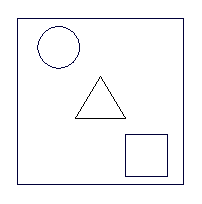
\includegraphics[width=40mm]{fig-sample.eps}
 \caption{\small{図の挿入例.}}
 \label{fig:sample}
\end{figure}

表についても同様に,label を付加し,本文から label を用いて参照する.
一例として,以下の表 \ref{tab:sample} をご参照いただきたい.

\begin{table}[H]
 \caption{\small{表の挿入例.}}
 \centering
 \begin{tabular}{|c|c|c|c|}
	\hline
		& 数学	& 英語	& 国語	\\ \hline
	太郎	& 68	& 91	& 34	\\
	次郎	& 53	& 12	& 97	\\ \hline
 \end{tabular}
 \label{tab:sample}
\end{table}

本サンプルでは,図表の出現が tex ファイルの記述箇所と同一となるように,
figure 環境や table 環境のオプションに「H」を用いているが,
このオプションは適宜変更しても構わない.

また,図表を一段組で大きく描画したい場合は,
figure 環境や table 環境の末尾にアスタリスクをつけた
「\verb+\begin{figure*} 〜 \end{figure*}+」や
「\verb+\begin{table*} 〜 \end{table*}+」を用いる.
図 \ref{fig:sample-big} でその例を示す.

\begin{figure*}[ht]
 \centering
 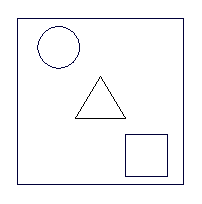
\includegraphics[width=80mm]{fig-sample.eps}
 \caption{\small{一段組での図の挿入例.}}
 \label{fig:sample-big}
\end{figure*}

\subsection{数式}
数式のインラインモードは \(x^2 + y^2 \leq 1\) のように表示させることができる.
インラインモードで「\verb+$...$+」を使うやり方は,
近年の LaTeX ではあまり推奨されていないが,その利用は妨げない.

ディスプレイ数式モードを利用する際に推奨するのは equation 環境である.
\begin{equation}
	\bA_p = \frac{\bA\cdot\bB}{|\bB|^2}\bB .
	\label{eq:samp1}
\end{equation}
数式の参照は「\verb+\ref+」ではなく「\verb+\eqref+」を用いる.
上記の数式を参照すると「式\eqref{eq:samp1}」となる.
このように,\verb+\eqref+ を用いた場合は数式中と同じ様式の括弧がつく.

また,複数行にわたる数式を表示したい場合は align 環境を用いることを推奨する.
以下の式\eqref{eq:samp2}にその例を示す.

\begin{align}
	& \begin{bmatrix}
	a_{11} & a_{12} & \cdots & a_{1n} \\
	a_{21} & a_{22} & \cdots & a_{2n} \\
	\vdots & \vdots & \ddots & \vdots \\
	a_{m1} & a_{m2} & \cdots & a_{mn} \\
	\end{bmatrix}
	\otimes
	\begin{bmatrix}
	b_{11} & b_{12} & \cdots & b_{1n} \\
	b_{21} & b_{22} & \cdots & b_{2n} \\
	\vdots & \vdots & \ddots & \vdots \\
	b_{m1} & b_{m2} & \cdots & b_{mn} \\
	\end{bmatrix} \notag \\
	& \qquad \qquad = \sum_{i}^{m}\sum_{j}^{n}a_{ij}b_{ij} .
	\label{eq:samp2}
\end{align}

eqnarray 環境は,最近の LaTeX では幾つかのパッケージと同時に利用すると
問題が発生することがあるため、利用は推奨しない.

\subsection{参考文献}
参考文献は本文の後に全部まとめて列挙する.
すべての参考文献は本文中で引用する.すべての参考文献には通し番号をつける.

本論文誌にはページ数の制限がないので,参考文献の数にも制限は設けない.
むしろ,\textbf{文献の引用数を節約せず,
論文の新規性を主張するに十分な参考文献を載せること.
特に,著者自身による関連発表の引用を怠らないこと. }

本稿の末尾に,英語論文と日本語論文の参考文献の一例 \cite{Ito04} を示す.
原則として,著者名,タイトル,掲載誌,(論文の場合には巻と号),
ページ数,発行年を記載すること.
著書の場合には,著書を特定する情報(出版社,ISBNなど)もできる限り記載すること.
なおウェブサイト等\cite{ArtScience}を引用する場合には,この限りではない.

本ファイルは\BibTeX を利用することを想定したサンプルとなっているが,
\BibTeX を利用せずに参考文献リストを記述する場合は,
「BibTeXを利用しない場合」と記されている箇所のコメントアウトされている部分を
参照のこと.

\subsection{著者略歴}

著者略歴は論文本体の最終行に,日本語であれば目安として200字以内,
英語の場合はそれと同程度の文章量で記述する.
内容は氏名のほか,出身(または在学)学校学部学科名や修了年次,職歴,
現職と職務,受賞,学位,主な研究分野,主な所属学会などを記載すること.
また,適切な大きさで顔写真を貼り付けること.
本稿の末尾に,その一例を示す.


% おわりに・まとめ

\section{まとめ}

本稿では,芸術科学会論文誌の投稿用のLaTeX版サンプルを提供した.
本サンプルに不具合が発生した場合には,
芸術科学会にご一報をいただけると非常に幸いである.


%%%%%%%%%%%%%%%%%%%%%%%%%%%%%%%%%%%%%%%%%%%%%%%%%%%%%%%%%%%%%%%%%%%%%%%%%%%%%%
%%% 参考文献

%% BibTeX を利用する場合.(利用しない場合は以下の2行をコメントアウト)

\bibliography{bibtex_samp} % BibTeX ファイル (.bib) を記述
\bibliographystyle{junsrt} % 番号を掲載順にソートする.

%% BibTeX を利用しない場合

%\begin{thebibliography}{99}
%
% \bibitem{Ito04}
% T. Itoh, Y. Yamaguchi, Y. Ikehata, Y. Kajinaga,
% Hierarchical Data Visualization Using a Fast Rectangle-Packing Algorithm,
% IEEE Transactions on Visualization and Computer Graphics,
% Vol. 10, No. 3, pp. 302-313, 2004.
%
% \bibitem{ArtScience}
% 芸術科学会,芸術科学会論文誌,http://art-science.org/journal/, 参照: 2014-12-10.
%
%\end{thebibliography}


\vspace{5mm}
%% BIOGRAPHY / 略歴

\noindent
\textbf{芸術科学 太郎}
\vspace{1mm} \\
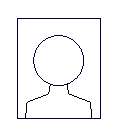
\includegraphics[width=25mm]{photo-face.eps} \\
1990年某大学理工学部電子通信学科卒業.
1992年某大学大学院理工学研究科電気工学専攻修士課程修了.
同年某社(株)入社.1997年博士(工学).
2000年米国某大学客員研究員.
2005年某社(株)退職,
2005年芸術科学大学大学院芸術科学研究科博士後期課程入学.
芸術と科学の接点に興味を持つ.
ACM, IEEE Computer Society, 芸術科学会,他会員.
%
\vspace{3mm}
\\
%
\textbf{芸術科学 次郎}
\vspace{1mm} \\
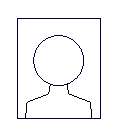
\includegraphics[width=25mm]{photo-face.eps} \\
1990年某大学理工学部電子通信学科卒業.
1992年某大学大学院理工学研究科電気工学専攻修士課程修了.
同年某社(株)入社.1997年博士(工学).
2000年米国某大学客員研究員.
2005年某社(株)退職,
2005年より芸術科学大学理学部情報科学科助教授,現在准教授.
芸術と科学の接点に興味を持つ.
ACM, IEEE Computer Society, 芸術科学会,他会員.
% ----



\end{document}
